\documentclass[conference,twocolumn]{IEEEtran}
\usepackage[backend=bibtex,firstinits=true]{biblatex}
\addbibresource{paper}
\makeatletter\def\blx@maxline{77}\makeatother

\newcommand{\comment}[1]{}
\newcommand{\numpc}[2]{\scriptsize #2\% {\tiny(#2)}}

\usepackage{graphicx}
\newcommand{\rb}[1]{\rotatebox{90}{#1}}

\usepackage{pifont}
\newcommand{\cmark}{\ding{51}}

\usepackage{hyperref}
\usepackage{mathtools}
\usepackage{booktabs}
\usepackage{multirow}
\usepackage{graphicx}

\title{Common Concerns in BYOD Policies}
\author{%
  \IEEEauthorblockN{Joseph Hallett}
  \IEEEauthorblockA{University of Edinburgh}
  \and
  \IEEEauthorblockN{David Aspinall}
  \IEEEauthorblockA{University of Edinburgh}
}

\begin{document}
\maketitle

\begin{abstract}
  Companies publish BYOD policies for employees to use their device at work.
  These policies are written using natural language, and vary in length and style.
  Using BYOD policies from five different sources we explore common concerns.
  Existing tools for enforcing policies has focussed on restricting app and device functionality.
  Our work looks at 5 BYOD policies and presents the common concerns and structures found in the policies themselves.
  This suggests where future MDM tools should focus their efforts.
\end{abstract}

\section{Introduction}
\label{sec:introduction}

Many employees bring their personal mobile devices to work.
To control the access these devices have, 70\% of companies publish \emph{bring your own device} (BYOD) policies~\cite{schulze_byod_2016}.
These BYOD policies are written documents for employees to read and follow.
They describe steps to take to secure devices appropriate to the workplace.
The policies say how employees should access data, and who should authorise decisions.

Companies have a variety of means to implement their policies.
Some companies may trust employees to follow the rules on their own.
Alternatively \emph{Mobile Device Management} (MDM) software can implement part of the policies: packages such as IBM's MaaS360 and Blackberry's offering~\cite{_ibm_????,_secure_????} can configure devices to restrict functionality and manage apps.
Research has looked at developing other tools such as UC-Droid~\cite{martinelli_enhancing_2016} or BYODroid~\cite{armando_enabling_2014} which was used to implement parts of a NATO BYOD policy~\cite{armando_developing_2016}.

Commercial tools are limited in what polices they can enforce.
The tools are limited to simple on-off configuration settings, and banning explicitly black-listed apps.
More sophisticated systems can use app-rewriting to recompile apps to tunnel traffic through a VPN, or geo-fencing to only apply policies in predefined areas.
These tools are not infallible.
One survey found that 50\% of companies with MDM software still had non-compliant devices in their networks~\cite{mobileiron_security_labs_q4_2015}.
Whilst app wrapping can protect some apps, in general it is ineffective~\cite{hao_effectiveness_2013}.

MDM software and research has, so far, focussed on restricting apps and device functionality.
But what are the concerns and restriction described in the policies themselves?
By analyzing 5 BYOD policies, we present the common concerns and structures found in the policies themselves.
The policies display varying styles for writing policies, and varying concerns.
In comparison to MDM software, the policies do not focus exclusively on restrictions but rather require employees acknowledge company rules and describe trust relationships between different departments.
This suggests there is little consensus on the best way to write such policies and that more research is needed.

\section{BYOD Policies}
\label{sec:byod_policies}

We analyzed 5 policies from different sources to find common concerns.
These five were chosen as they come from a variety of sources and industries.
Two are advisory, published specialist institutions to help other companies implement their own policies.
Three are policies used in a hospital, a company selling emergency sirens, and a university.
\begin{itemize}
  \item The SANS policy~\cite{nicholas_r._c._guerin_security_2008} is a hypothetical BYOD policy that a company could use as a starting point to base its own policy on.
    It is prescriptive and long, focussed on technical restrictions such as disabling device features.
  \item The HiMSS policy~\cite{healthcare_information_and_management_systems_society_mobile_2012} also is a hypothetical policy, for US hospital trusts planing to implement a BYOD policy.
    It is short, but and written from the perspective of the employee agreeing to the policy.
    This is different to the other policies where instead the policy is written as rules for employees to follow.
  \item The NHS policy~\cite{kennington_mobiles_2014} is a BYOD policy used in a British hospital trust.
    It is long, and describes a complex policy in a large organization with a complex hierarchy.
  \item The final two policies are simpler, the fourth is taken from a company selling emergency sirens for cars~\cite{code3pse.org_sample_????}, the fifth is by the University of Edinburgh.  
\end{itemize}
Both are short, relatively uncomplicated, but typical examples of policies found \emph{in the wild}.

Not all of the policies are written in the same style.
Most are written from the perspective of a company or IT department telling an employee what to do.
The HiMSS policy, however, is written as a contract where the user tells the company how they will behave.
Most policies separate individual policy rules into small individual rules each which must be followed.
The Edinburgh policy groups them together into two or three large rules, with different increasing sets of sub-rules for low and high risk employees to follow.

To help compare the policies, they were first translated them into a formal language~\cite{hallett_specifying_2016}.
We use a dialect of SecPAL~\cite{becker_secpal:_2010} that we used for describing app privacy preferences~\cite{hallett_apppal_2016}.
SecPAL is designed to be readable, and requires an explicit authority to \emph{speak} individual statements.
This allows SecPAL-based languages to capture delegation relationships and the differences in style between the policies.
Both the formalization of the policies\footnote{\url{https://github.com/apppal/apppal-byod-policy-translations}} and tooling for our variant of SecPAL\footnote{\url{https://github.com/apppal/libapppal}} are available online.

\section{Rule Structures}

Each of the policies are split into a series of rules.
The SecPAL assertions we used to translate the rules have a common structure, similar to Datalog.
An authority (the speaker) will decide that a fact is true, if it can be convinced of a series of conditional facts are also true. 

\begin{center}\ttfamily\footnotesize%
  \newcommand{\sptoken}[1]{$\langle\text{#1}\rangle$}
  \sptoken{speaker} says $\overbrace{\text{\sptoken{X} \sptoken{\sf predicate}}}^{\text{\sf fact}}$ if $\overbrace{\text{\sptoken{Y} \sptoken{predicate}}}^{\text{condition}}\cdots$.
\end{center}

The predicates used to describe decisions made by the rules fall into 4 categories.
\emph{Can} predicates describe what their subjects can do; for instance whether a device can connect to a server.
\emph{Must} predicates describe obligations, such as reporting a lost device.
\emph{Has} predicates ensure an action has been completed in the past, such as approving an app.
Finally \emph{is} predicates describe a typing property about their subjects.

The occurrence of each type of predicate in each policy is shown in \autoref{tab:prefix}.
The use of each type is also split by whether the predicate is a \emph{decision} made by the policy, or a \emph{condition} for making that decision.
\emph{Can} and \emph{must} decisions feature in all policies excepting \emph{can} decisions in the Edinburgh policy, in part due to the structure of the policy as discussed in \autoref{sec:introduction}.
This is expected, these are access control decisions and reactions to events; both topics that existing MDM tools have focussed on implementing.
\emph{Has} and \emph{is} predicates are the majority of the conditions, but there are also decisions using them too.

\comment{
  This suggests that implementing a policy is more complex than choosing what a predefined group of devices can or cannot do.
  The groups themselves are defined by policy rules that can dynamically change based on the policy.
  Existing MDM tools, such as MaaS360, do not allow for policies to be applied based on the basis of policies.
}
Existing MDM tools present policies as a series of tick-boxes for what a device \emph{can} and \emph{must} do~(\autoref{fig:policy}).
An administrator selects which policies each device must follow, a predominantly manual process.
In our examination of the policies, as well as finding rules that describe what a device \emph{can} do, we find rules that group devices by what they \emph{have} or \emph{are}.
Selecting which restrictions to apply to a device is defined by policies; but existing MDM tools do not allow policies to be selected on the basis of policies.
MDM tools perhaps need greater flexibility to fully implement all aspects of a BYOD policy.


\begin{table}\sffamily\footnotesize\centering
  \newcommand{\zilch}[0]{\scriptsize 0}
  \setlength{\tabcolsep}{1pt}
\begin{tabular}{ c  c c c c c c c c c }
\toprule
             & \multicolumn{4}{c}{Decision}                                                    && \multicolumn{4}{c}{Condition} \\
Policy       & \rb{Can}                     & \rb{Must}      & \rb{Has}       & \rb{Is}        && \rb{Can}      & \rb{Must}     & \rb{Has}        & \rb{Is}        \\
\midrule
SANS         & \numpc{26}{35}               & \numpc{22}{29} & \numpc{7 }{9 } & \numpc{20}{27} && \numpc{2 }{2} & \numpc{2 }{2} & \numpc{8 }{8}   & \numpc{81}{87} \\
HiMSS        & \numpc{6 }{21}               & \numpc{12}{41} & \numpc{9 }{31} & \numpc{2 }{7 } && \zilch        & \zilch        & \numpc{3 }{13}  & \numpc{20}{87} \\
NHS          & \numpc{13}{19}               & \numpc{18}{26} & \numpc{23}{33} & \numpc{16}{23} && \numpc{2 }{2} & \zilch        & \numpc{20}{19}  & \numpc{83}{83} \\
Sirens       & \numpc{12}{27}               & \numpc{20}{45} & \numpc{5 }{11} & \numpc{7 }{16} && \numpc{1 }{2} & \numpc{4 }{7} & \numpc{1 }{2}   & \numpc{50}{89} \\
Edinburgh    & \zilch                       & \numpc{2 }{18} & \numpc{9 }{82} & \zilch         && \numpc{2 }{7} & \numpc{2 }{7} & \numpc{15}{ 50} & \numpc{11}{37} \\
\bottomrule \\
\end{tabular}
\caption{Occurrences of predicate-types in each policy.}
\label{tab:prefix}
\end{table}

\begin{figure}
  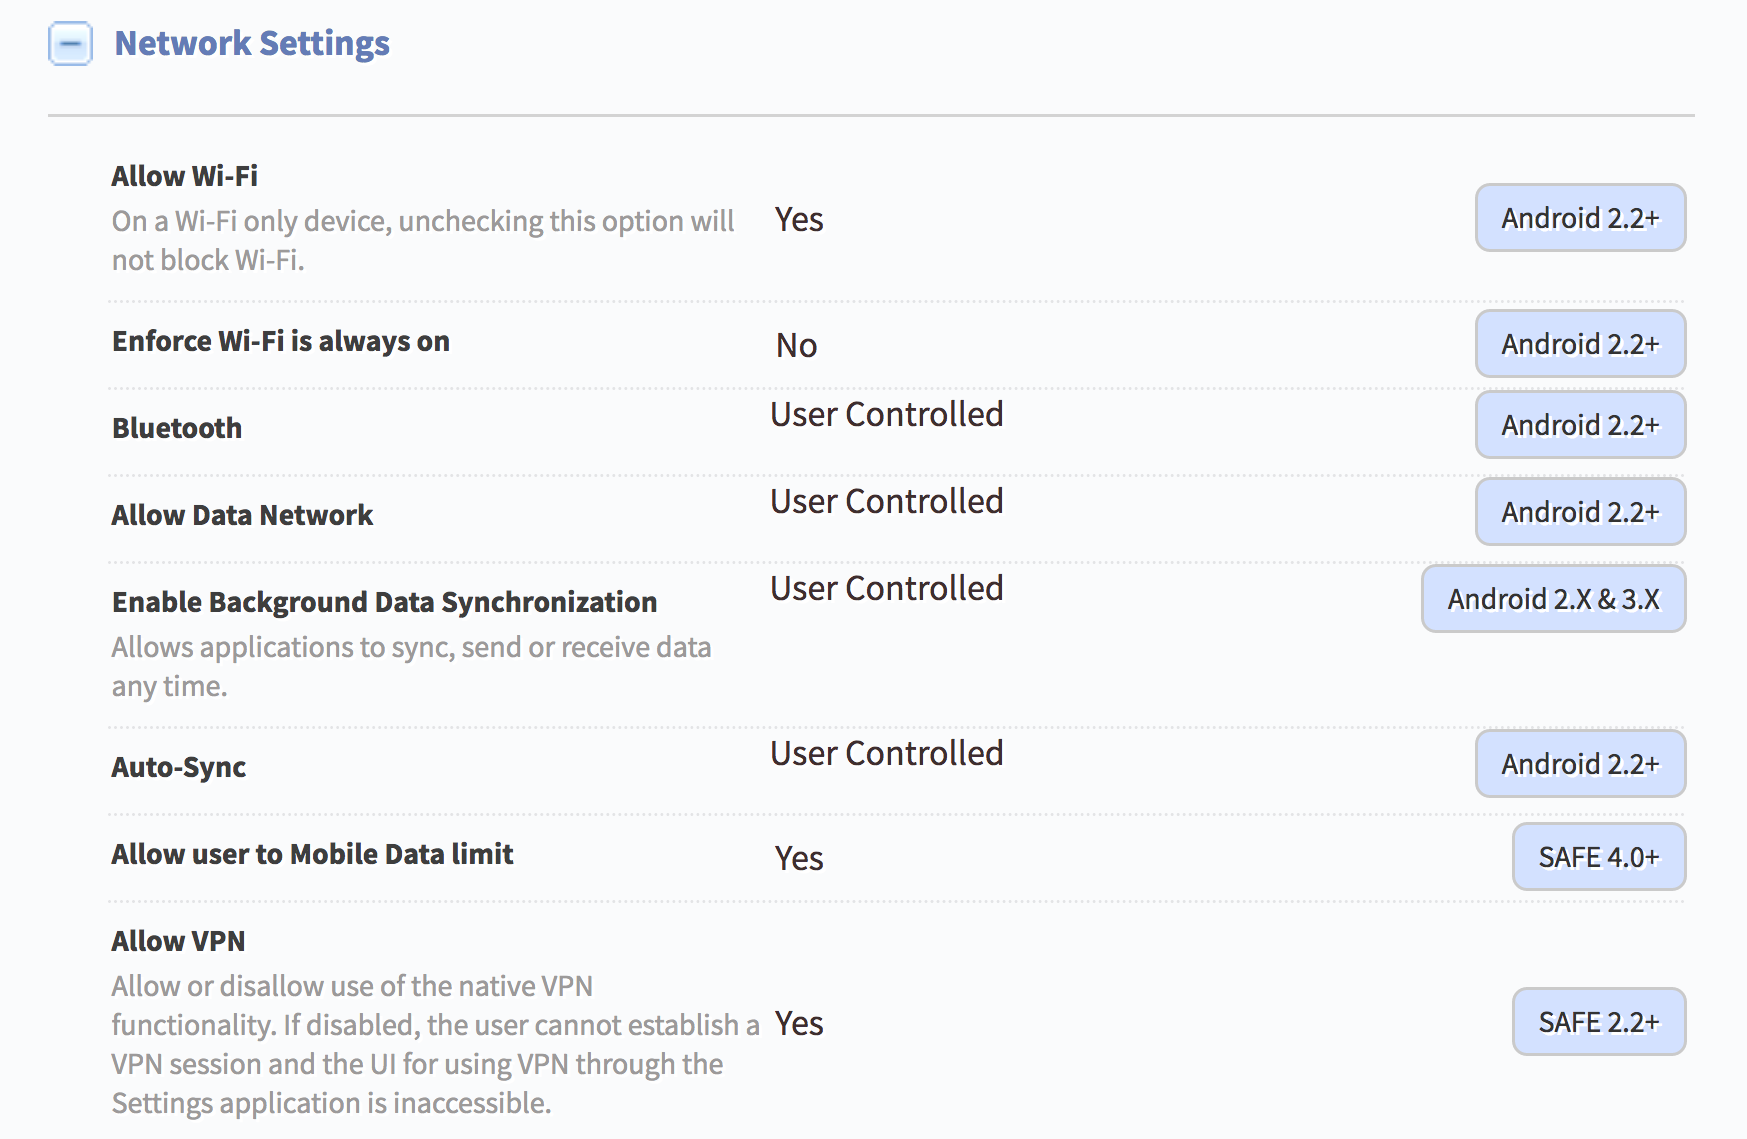
\includegraphics[width=\linewidth]{maas360-policy.png}
  \caption{Example policy from the MaaS360 MDM software.}
  \label{fig:policy}
\end{figure}

\section{Common Concerns and Checks}
\label{sec:common_concerns}

Analyzing each of the policies common concerns become apparent.
%We took care to ensure that our policies used the same predicates between themselves.
A summary of predicates, with the same meaning, used in multiple policies by our translation is given in \autoref{tab:common}.


Acknowledgements, where individuals are asked to acknowledge other policies, and predicates linking devices to owners are used in all policies.
Most policies described rules for when device features should be enabled and disabled.
Configuring device features is a common feature to many MDM packages, but tracking what a user agrees to is not seen in leading MDM packages like MaaS360 or BES~\cite{rob_smith_magic_2016}.
Only 2 out of 5 policies had rules limiting what networks, servers, or access points a device could access;
  and only the two most complex policies had rules limiting what apps could be installed.
This is surprising as a common feature of MDM tools is controlling how devices and apps access networks.
Users have privacy preferences about apps~\cite{lin_modeling_2014}, but not all companies try and control what apps employees install.
Providing curated app stores and blacklisting apps is a feature common to many MDM programs.
Not all policies express rules about which apps to install, however.

\begin{table}\sffamily\footnotesize\centering
\begin{tabular}{c c c c c c}
\toprule                        \\ 
Predicate                       & \rb{SANS} & \rb{HiMSS} & \rb{NHS} & \rb{Sirens} & \rb{Edinburgh} \\
\midrule
\comment 5  mustAcknowledged    &    \cmark & \cmark     &   \cmark & \cmark      &         \cmark \\
\comment 5  hasAcknowledged     &    \cmark & \cmark     &   \cmark & \cmark      &         \cmark \\
\comment 5  isOwnedBy           &    \cmark & \cmark     &   \cmark & \cmark      &         \cmark \\
\comment 5  isDevice            &    \cmark & \cmark     &   \cmark & \cmark      &         \cmark \\
\comment 4  mustDisable         &    \cmark &            &   \cmark & \cmark      &         \cmark \\
\comment 4  isLost              &    \cmark & \cmark     &   \cmark & \cmark      &                \\
\comment 4  isEmployee          &    \cmark &            &   \cmark & \cmark      &         \cmark \\
\comment 4  isApp               &    \cmark & \cmark     &   \cmark & \cmark      &                \\
\comment 4  isActivated         &    \cmark & \cmark     &   \cmark &             &         \cmark \\
\comment 3  mustEnable          &    \cmark & \cmark     &          & \cmark      &                \\
\comment 3  mustWipe            &           & \cmark     &   \cmark & \cmark      &                \\
\comment 3  isEncrypted         &    \cmark &            &   \cmark &             &         \cmark \\
\comment 3  hasMet              &    \cmark &            &   \cmark &             &         \cmark \\
\comment 3  canMonitor          &    \cmark &            &   \cmark & \cmark      &                \\
\comment 2  mustInform          &    \cmark &            &   \cmark &             &                \\
\comment 2  isTelephoneNumber   &    \cmark &            &   \cmark &             &                \\
\comment 2  isString            &           &            &   \cmark & \cmark      &                \\
\comment 2  isSecurityLevel     &    \cmark & \cmark     &          &             &                \\
\comment 2  isInstallable       &    \cmark &            &   \cmark &             &                \\
\comment 2  isFeature           &    \cmark &            &          & \cmark      &                \\
\comment 2  isData              &    \cmark &            &          & \cmark      &                \\
\comment 2  isApprovedFor       &           & \cmark     &   \cmark &             &                \\
\comment 2  isApproved          &    \cmark & \cmark     &          &             &                \\
\comment 2  hasFeature          &           &            &   \cmark &             &         \cmark \\
\comment 2  hasDevice           &           & \cmark     &   \cmark &             &                \\
\comment 2  hasDepartment       &           & \cmark     &          &             &         \cmark \\
\comment 2  canUse              &    \cmark &            &   \cmark &             &                \\
\comment 2  canStore            &    \cmark & \cmark     &          &             &                \\
\comment 2  canInstall          &    \cmark &            &   \cmark &             &                \\
\comment 2  canConnectToServer  &    \cmark &            &   \cmark &             &                \\
\comment 2  canConnectToNetwork &    \cmark &            &          & \cmark      &                \\
\comment 2  canConnectToAP      &    \cmark & \cmark     &          &             &                \\
\comment 2  canCall             &    \cmark &            &   \cmark &             &                \\
\comment 2  canBackupTo         &           & \cmark     &          &             &         \cmark \\
\bottomrule                     \\
\end{tabular}
\caption{Occurrences of predicates common to multiple policies.}
\label{tab:common}
\end{table}

All of the policies we looked at required employees to be aware of and acknowledge the existence of other policies.
The use of acknowledgements is noteworthy because policies acknowledged may not be ones that are enforcible automatically.
These other rules include ethical or legal guidelines and disclaimers about data-loss.
Writing software to check a user is aware they may lose the data, and is behaving ethically may not be possible.

An aspect of acknowledgements is that they require a delegation of trust from the company to their employees.
The employees have to be responsible for stating what they do or do not acknowledge.
Delegation is key to other policy decisions in the policies.
The IT department is delegated to audit apps.
Users are responsible for reporting their device missing.

We summarise the number (and percentage) of rules in the policies using acknowledgements and delegation relationships in \autoref{tab:summary}.
For comparison we also give the at the number of rules which describe some form of restriction.
Delegation relationships form a significant proportion of all the policies.
Acknowledgements are used extensively in the HiMSS policy, but rarely in the SANS policy.
Overall acknowledgements form as much a part of the policies as do device restrictions.
MDM software has focussed on implementing device restrictions and configurations; but it would seem that other aspects are equally important.

\begin{table}\centering\footnotesize\sffamily
  \setlength{\tabcolsep}{1pt}
  \begin{tabular}{l c c c c c}
    \toprule
                                   & \rb{SANS}      & \rb{HiMSS}     & \rb{NHS}       & \rb{Sirens}    & \rb{Edinburgh} \\
    \midrule                                                                                          
    Rules in policy                & 33             & 15             & 56             & 20             & 25             \\
    \midrule                                                                                          
    Rules using acknowledgement    & \numpc{2}{6}   & \numpc{10}{67} & \numpc{11}{20} & \numpc{6}{24}  & \numpc{1}{5}   \\
    Rules using delegation         & \numpc{23}{70} & \numpc{5}{33}  & \numpc{33}{59} & \numpc{13}{52} & \numpc{2}{10}  \\
    Rules describing a restriction & \numpc{18}{54} & \numpc{3}{20}  & \numpc{8}{14}  & \numpc{5}{20}  & \numpc{1}{5}   \\
    \bottomrule                    \\
  \end{tabular}
  \caption{Summary of idioms in each of the policies.}
  \label{tab:summary}
\end{table}

\section{Principals and Delegation}

Each of the policies use delegation to describe rules.
A delegation requires at least two parties: someone to hand off the decision, and someone to hand the decision to.
They can be individuals, but often they are a role that several individuals may fulfill
SecPAL requires each assertion to be made by an explicit authority.
When translating the policies into SecPAL we created a principal to deliver the policy.
In most cases we took the company (who had authored the document) as the speaker. 
In the HiMSS policy, however, rules are phrased as a user stating what they will do.

In most policies we found three speakers were making the bulk of the decisions.
A primary speaker expresses the bulk of the policy and delegation relationships.
A technical user expresses sub-policies and makes specific decisions (is an app part of the standard company apps for instance).

\begin{table}\centering\footnotesize\sffamily
  \begin{tabular}{c l l}
    \toprule
    \multirow{4}{*}{\rb{SANS}}       & Speakers          & 10                \\
                                     & Primary Speaker   & company           \\
                                     & Technical Speaker & it-department     \\
                                     & User speaker      & user              \\
    \midrule
    \multirow{4}{*}{\rb{HiMSS}}      & Speakers          & 3                 \\
                                     & Primary Speaker   & user              \\
                                     & Technical Speaker & xyz-health-system \\
                                     & User speaker      & department        \\
    \midrule
    \multirow{4}{*}{\rb{NHS}}        & Speakers          & 11                \\
                                     & Primary Speaker   & nhs-trust         \\
                                     & Technical Speaker & it-department     \\
                                     & User speaker      & staff             \\
    \midrule
    \multirow{4}{*}{\rb{Sirens}}     & Speakers          & 4                 \\
                                     & Primary Speaker   & department        \\
                                     & Technical Speaker & it-department     \\
                                     & User speaker      & employee          \\
    \midrule
    \multirow{4}{*}{\rb{Edinburgh}}  & Speakers          & 2                 \\
                                     & Primary Speaker   & records-management\\
                                     & Technical Speaker &                   \\
                                     & User speaker      & employee          \\
    \bottomrule                     \\
  \end{tabular}
  \caption{Summary of different principals in policies.}
  \label{tab:principals}
\end{table}

\section{Conclusions}
\label{sec:conclusions}

\begin{itemize}
  \item Our formalisation of the policies is subjective.
  \item Remarks about lack of commonality.
\end{itemize}

\printbibliography{}
\end{document}
